\subsection{UC3 - Tracciamento PRESENZE\textsubscript{G} in sede}
\begin{itemize}
    \item \textbf{Identificativo}: UC3
    \item \textbf{Nome}: Tracciamento PRESENZE\textsubscript{G} in sede
    \item \textbf{Descrione grafica}:
\end{itemize}
\begin{center}
    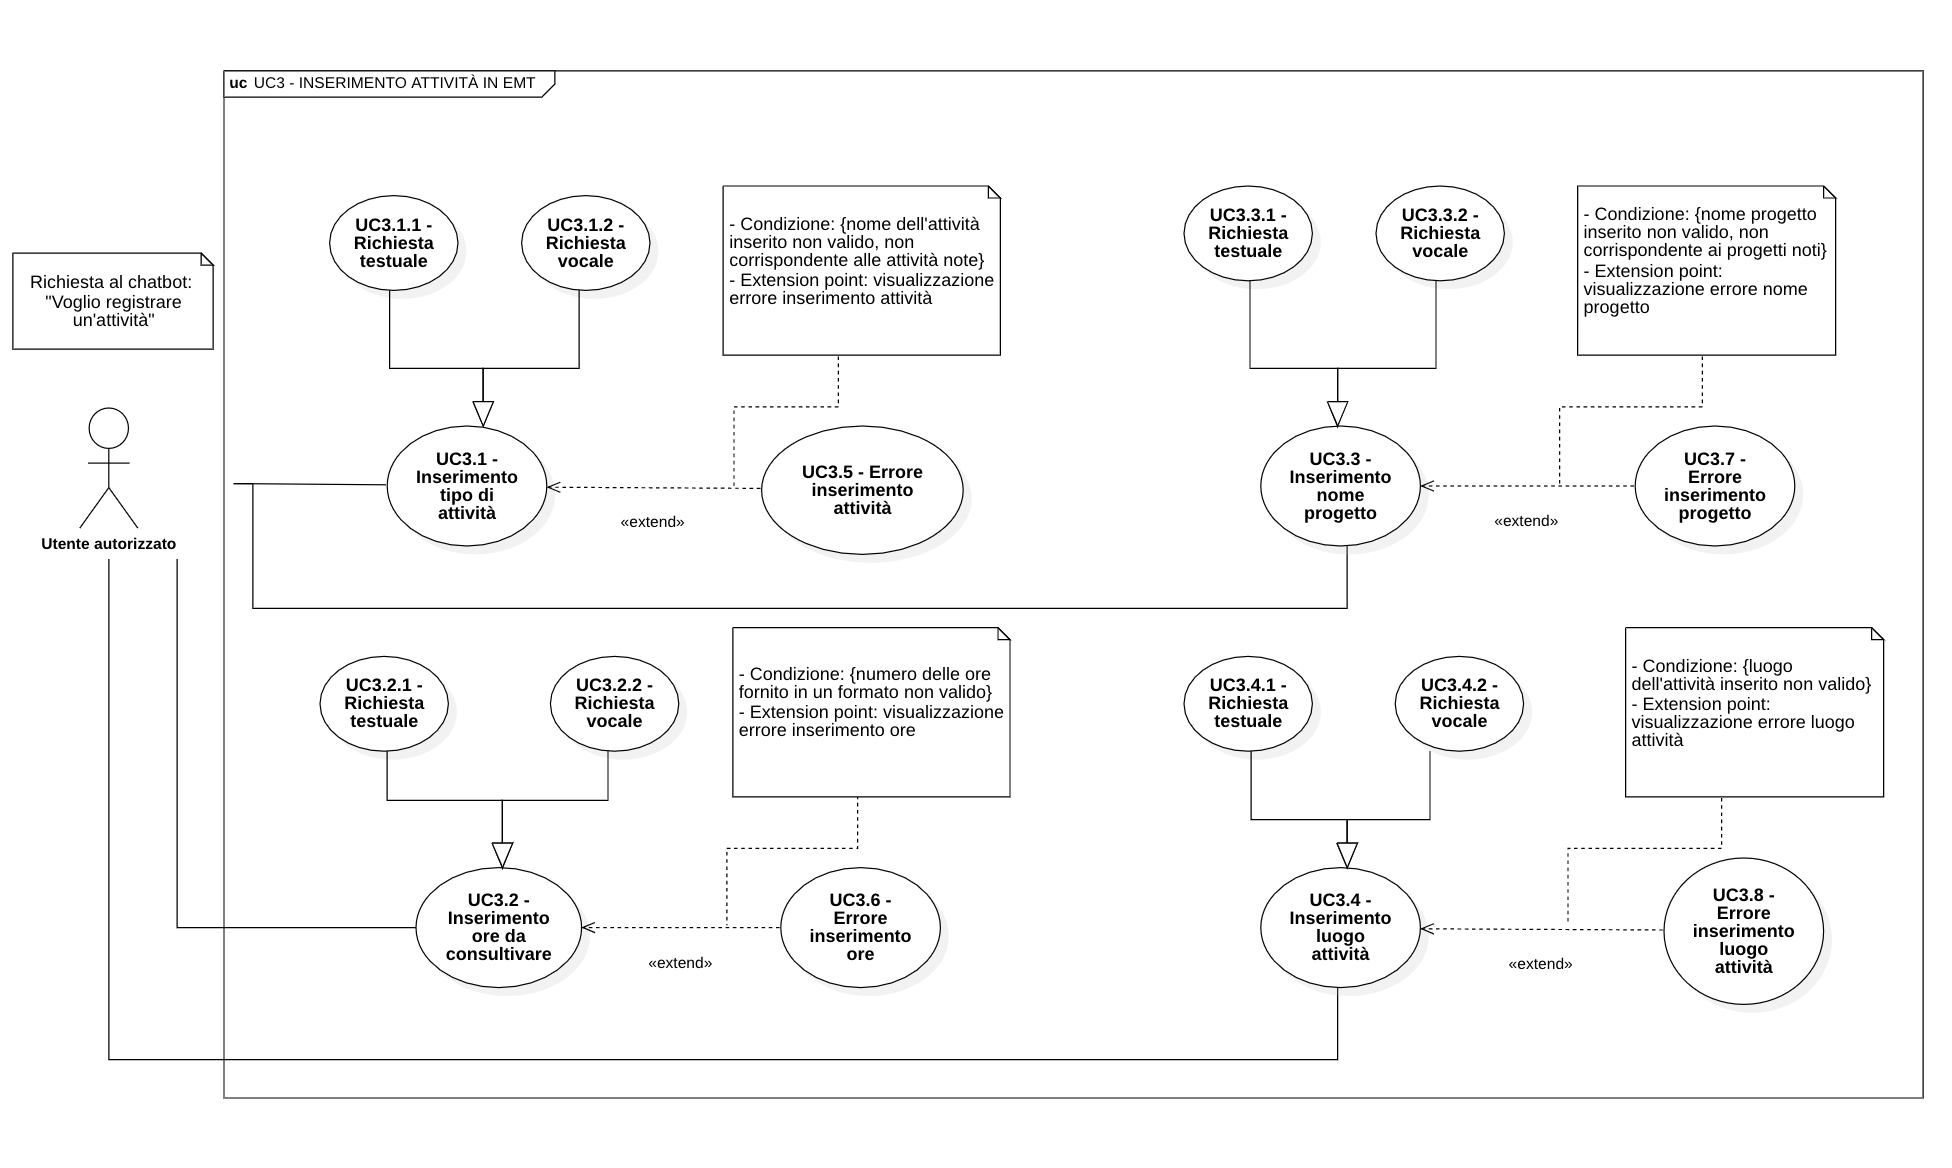
\includegraphics[scale=0.50]{images/UC3.png} 
\end{center}
\begin{itemize}
    \item \textbf{Attori}
 \begin{itemize} 
    \item \textit{Primari}: utente autorizzato
    \item \textit{Secondari}: non presenti
 \end{itemize}
 \item \textbf{Precondizione}: l'utente ha superato con successo la fase di autenticazione e vuole registrare la sua presenza in sede. 
 \item \textbf{Postcondizione}: l'utente è riuscito a registrare con successo la sua presenza in sede. 
 \item \textbf{Scenario principale}: L'utente comunica al chatbot la richiesta di voler registrare la sua presenza presso la sede \textit{XYZ} specificato in UC3.1. Si possono verificare degli scenari secondari che non portano al compimento di tale operazione, tra cui:
    \begin{itemize}
        \item Il chatbot non è in grado di interpetare la richiesta fatta dall'utente. (UC2)
        \item Durante l'esecuzione dell'azione richiesta si è verificato un errore. (UC14)
        \item La sede indicata dall'utente non esiste. (UC18)
    \end{itemize}
\end{itemize}
\newpage

\subsubsection{UC3.1 - Inserimento nome sede}
\begin{itemize}
    \item \textbf{Identificativo}: UC3.1
    \item \textbf{Nome}: Inserimento nome sede
    \item \textbf{Descrione grafica}: (approfondita in UC3)
    \item \textbf{Attori}
 \begin{itemize} 
    \item \textit{Primari}: utente autorizzato
    \item \textit{Secondari}: non presenti
 \end{itemize}
 \item \textbf{Precondizione}: l'utente ha espresso la sua volontà al chatbot di procedere con l'operazione di registrazione della presenza in una sede.
 \item \textbf{Postcondizione}: l'utente comunica al chatbot la sede presso la quale effettuare la registrazione.
 \item \textbf{Scenario principale}: l'utente inserisce l'indirizzo identificato della sede presso la quale si vuole registrare in maniera testuale (UC3.1.1) oppure vocale (UC3.1.2). La presenza viene successivamente registrata con successo o l'utente ha inserito un indirizzo non valido provocando un messaggio di errore (UC3.2). 
\end{itemize}

\subsubsection{UC3.2 - Visualizzazione errore sede}
\begin{itemize}
    \item \textbf{Identificativo}: UC3.2
    \item \textbf{Nome}: Visualizzazione errore sede
    \item \textbf{Descrione grafica}: (approfondita in UC3)
    \item \textbf{Attori}
 \begin{itemize} 
    \item \textit{Primari}: utente autorizzato
    \item \textit{Secondari}: non presenti
 \end{itemize}
 \item \textbf{Precondizione}: l'utente ha fornito al chatbot un indirizzo di una sede non valido.
 \item \textbf{Postcondizione}: il chatbot mostra all'utente un messaggio di errore relativo alla non validità dell'indirizzo fornito, consigliando di ripetere la procedura. 
 \item \textbf{Scenario principale}: l'utente inserisce in maniera testuale (UC3.1.1) oppure vocale (UC3.1.2) un indirizzo di una sede non valido, di conseguenza il chatbot comunica un messaggio di errore e invita l'utente a riprovare. 
\end{itemize}